\documentclass[10pt,landscape,a4paper]{article}
\usepackage[utf8]{inputenc}
\usepackage[english]{babel}
\usepackage[utopia,sfscaled]{mathdesign}
\usepackage{multicol}
\usepackage[top=2mm,bottom=2mm,left=2mm,right=2mm]{geometry}
\usepackage{lipsum}
\usepackage[framemethod=tikz]{mdframed}
\usepackage{microtype}
\usepackage{graphicx}
\usepackage{amsmath}
\usepackage{breqn}
\usepackage{enumitem}
\usepackage{titlesec}

\setitemize{noitemsep,topsep=0pt,parsep=0pt,partopsep=0pt}
\setenumerate{noitemsep,topsep=0pt,parsep=0pt,partopsep=0pt}
\setlength{\parindent}{0pt}
\setlength{\parskip}{0.2\baselineskip}
\titleformat*{\section}{\footnotesize\bfseries}
\titleformat*{\subsection}{\scriptsize\bfseries}
\titlespacing{\section}{0pt}{\parskip}{-\parskip}
\titlespacing{\subsection}{0pt}{\parskip}{-\parskip}

\graphicspath{{images/}}

\DeclareMathOperator*{\argmin}{argmin}
\DeclareMathOperator*{\argmax}{argmax}

\begin{document}
\tiny
\begin{multicols*}{5}
\section{Validation}
% TODO: 2016_valid Q1 pseudocode

Validation Techniques:
\begin{itemize}
    \item fixed-validation:
    \begin{itemize}
        \item fixed sizes of train dataset and validation dataset
    \end{itemize}
    \item k-fold validation:
    \begin{itemize}
        \item divide dataset into \(k\) parts
        \item use \(k-1\) parts for training and the other part for validation
        \item repeat \(k\) times then average
    \end{itemize}
    \item loop validation (leave-one-out validation):
    \begin{itemize}
        \item use all dataset for training but leave one object for validation
        \item repeat \(n\) times then average
    \end{itemize}
\end{itemize}
Model Selection:
\begin{itemize}
    \item optimization bias is small when a few models are compared
    \item optimization bias is large when a lot of models are compared
\end{itemize}


\section{Parametric \& Non-Parametric}
\begin{itemize}
    \item parametric
    \begin{itemize}
        \item fixed \# parameters
        \item more data doesn't help
    \end{itemize}
    \item non-parametric
    \begin{itemize}
        \item \# parameters grows with \(n\)
        \item more data \(\rightarrow \)  more complicated
    \end{itemize}
    \item examples:
    \begin{itemize}
        \item k-means (non-parameters)
        \item softmax multi-class classification (parametric)
        \item PCA (parametric)
        \item neural networks (parametric)
    \end{itemize}
\end{itemize}

\section{Data Standardization}
\begin{itemize}
    \item \(\mu \) = mean of \(X_j\) and \(y\), \(\sigma \) = std of \(X_j\) and \(y\)
    \item \(x_i = x_i - \frac{\mu}{\sigma}\)
    \item use the \(\mu \) and \(\sigma \) from training data on test data
\end{itemize}

\section{Feature Selection}

Note:
Regression Weights vs. Search and score
\begin{itemize}
    \item pro: fast
    \item con: may drop import features if collinear
\end{itemize}

\section{Trees}

\subsection{Decision Tree}
Decision Stump: (\(n\) objects, \(d\) features, \(t\) thresholds)
\begin{itemize}
    \item cost:
    \begin{itemize}
        \item cost: \(O(ndt)\) (without sorting, computing score for \(dt\) rules)
        \item cost: \(O(n^2d)\) (consider only features)
        \item cost: \(O(nd \log(n))\) (with sorting, sorting costs \(O(n \log(n))\) per feature)
    \end{itemize}
\end{itemize}

\section{Naïve Bayes}
\begin{align*}
    p(y_i|x_i) &= \frac{p(x_i|y_i) p(y_i)}{p(x_i)} \\
    &\propto p(x_i|y_i) p(y_i) \\
    &\approx \prod_{j=1}^{d} (p(x_{ij}|y_i)) p(y_i)
\end{align*}
\begin{equation*}
    p(\hat{y} = 1|\hat{x}) > p(\hat{y}=0|\hat{x}) \Rightarrow \hat{y} = 1
\end{equation*}
Laplace Smoothing:\(\frac{(\text{\# spam messages with } x_i)+1}{(\text{\# spam messages})+2}\)

\section{Clustering}

Note: \\
Density-Based vs. K-Means:
\begin{itemize}
    \item pros:
    \begin{itemize}
        \item don't need to pre-specify \# clusters
    \end{itemize}
    \item cons:
    \begin{itemize}
        \item no loss function interpretation
        \item two hyper parameters to set
        \item slower \& more complicated
    \end{itemize}
\end{itemize}

\section{Kernels}

Note: \\
RBF Kernels vs. Linear Kernels:
\begin{itemize}
    \item pro: fit more complicated shape
    \item con: danger of overfitting
\end{itemize}

\section{Gradient Descent}

\subsection{Stochastic Gradient Descent}

Note:
\begin{itemize}
    \item minibatch size \(\downarrow \) \(\rightarrow \) each iteration is faster, but more iterations needed
\end{itemize}

\section{PCA}
Objective Function:
\begin{align*}
    f(W,Z) &= \sum_{i=1}^{n} \sum_{j=1}^{d} (w_j^\intercal z_i - x_{ij})^2 \\
    &= \sum_{i=1}^{n} ||W^\intercal z_i - x_i||^2 \\
    &= ||ZW-X||_F^2
\end{align*}
Matrix Factorization: \(X_{n \times d} \approx Z_{n \times k} W_{k \times d}\) \\
% \begin{dmath*}
%     f(W,Z) = \sum_{i=1}^{n} \sum_{j=1}^{d} (w_j^\intercal z_i - x_{ij})^2 + \frac{\lambda_W}{2} ||W|_F^2 \frac{\lambda_Z}{2} ||Z||_F^2
% \end{dmath*}
Alternating Minimization:
\begin{itemize}
    \item \(\nabla_W f(W,Z) = Z^\intercal Z W - Z^\intercal X\),so \(W = (Z^\intercal Z)^{-1} (Z^\intercal X)\)
    \item \(\nabla_Z f(W,Z) = Z W W^\intercal - X W^\intercal \), so \(Z = X W^\intercal (W W^\intercal)^{-1}\)
    \item find local optimum but not global optimum (sensitive to initialization)
    \item local optimum become global optimum if randomly initialize \(W\) and \(Z\)
    \item not jointly convex --- different \(W\) and \(Z\) depending on initialization
\end{itemize}
Stochastic Gradient:
\begin{itemize}
    \item \(w_j^{t+1} = w_j^t - \sigma_t \nabla_{w_i} f(w_j,z_i,x_{ij})\)
    \item \(z_i^{t+1} = z_i^t - \sigma_t \nabla_{z_i} f(w_j,z_i,x_{ij})\)
    \item where \(f(w_j,z_i,x_{ij}) = (w_j^t z_i - x_{ij})^2\)
\end{itemize}
Variance Explained: \(1 - \frac{||ZW-X||_F^2}{||X||_F^2}\) \\
Prediction Phase:
\begin{enumerate}
    \item center test data
    \item compute \(\hat{Z} = \hat{X} W^\intercal (W W^\intercal)^{-1}\)
\end{enumerate}
Trade-off:
\begin{itemize}
    \item reduce overfitting when \emph{both} W and Z are regularized
    % TODO: 2016 Final Q8 (d)
    % TODO: L29 s7a
\end{itemize}
PCA is not unique (e.g. \(ZW = (-Z)(-W)\)): \(\because\)
\begin{itemize}
    \item can multiply any \(W_c\) by any non-zero \(\sigma\)
    \item can rotate any \(W_c\) arbitrarily within the span
    \item can switch any \(W_c\) with another \(W_c'\)
\end{itemize}
Make PCA Unique:
\begin{itemize}
    \item Normalization: \(||W_1|| = 1\) and \(||W_2|| = 1\)
    \item Orthogonality: \(W_1^\intercal W_2 = 0\) (perpendicular)
\end{itemize}
Applications: outlier detection, dimensionality reduction, data compression, features for linear models, visualization, factor discovery, filling in missing entries \\

\subsection{Non-Negative Matrix Factorization (NMF)}
NMF
\begin{itemize}
    \item leads to sparsity
    \item regularizes \(W\)
\end{itemize}
Projected Gradient:
\begin{enumerate}
    \item \(w^{t+\frac{1}{2}} = w^t - \sigma^t \nabla f(w^t)\)
    \item \(w_j^{t+1} = \max \{0, w_j^{t+\frac{1}{2}}\} \)
    \item repeat
\end{enumerate}
Ways to Use Projected Gradient:
\begin{itemize}
    \item alternate between projected gradient steps between \(W\) and \(Z\)
    \item run projected gradient on both at once
    \item sample random \(i\) and \(j\) and do \emph{stochastic} gradient descent
\end{itemize}
Problems of NMF:
\begin{itemize}
    \item non-convex
    \item sensitive to initialization
    \item hard to find global optimum
\end{itemize}

\subsection{Variants of PCA}
L2-regularized PCA:
\begin{dmath*}
    f(W,Z) = \frac{1}{2} ||ZW-X||_F^2 + \frac{\lambda_1}{2} ||W||_F^2 + \frac{\lambda_2}{2} ||Z||_F^2
\end{dmath*}
\begin{itemize}
    \item need to regularize \emph{both} \(W\) and \(Z\) otherwise one will compensate the other
\end{itemize}
L1-regularized PCA:
\begin{dmath*}
    f(W,Z) = \frac{1}{2} ||ZW-X||_F^2 + \frac{\lambda_1}{2} \sum_{i=1}^{n} ||z_i||_1 + \frac{\lambda_2}{2} \sum_{j=1}^{d} ||w_j||_1
\end{dmath*}
\begin{itemize}
    \item pros:
    \begin{itemize}
        \item negative coefficients usually make sense
        \item can set \(\lambda_1\) and \(\lambda_2\) to control sparsity
    \end{itemize}
    \item con: need to set \(\lambda_1\) and \(\lambda_2\)
    \item L1 on \(Z\) = sparse coding, L1 on \(W\) = sparse dictionary learning
\end{itemize}

\subsection{Robust PCA}
\begin{dmath*}
    f(W,Z) = \sum\limits_{i=1}^{n} \sum\limits_{j=1}^{d} |w_j^\intercal z_i - x_{ij}| + \frac{\lambda_1}{2} \sum\limits_{i=1}^{n} \sum\limits_{c=1}^{k} z_{ic}^2 + \frac{\lambda_2}{2} \sum\limits_{j=1}^{d} \sum\limits_{c=1}^{k} |w_{cj}|
\end{dmath*}
\begin{itemize}
    \item absolute loss \(\rightarrow \) robust to outliers
    \item encourages residuals to be exactly 0
    \item L2-regularization works when both \(W\) and \(Z\) are regularized
    \item L1-regularization gives spars latent factors/features
    \item logistic/softmax/Poisson losses for discrete \(x_{ij}\)
    \item change of basis for non-linear latent-factor models
\end{itemize}

\subsection{Note}
ISOMAP vs. PCA
\begin{itemize}
    \item pro: can learn non-linear projections (e.g. manifold)
    \item con: more expensive, don't get basis interpretation
\end{itemize}
NMF vs. PCA
\begin{itemize}
    \item pro: sparsity, more interpretable in some cases
    \item con: more expensive, worse reconstructions
\end{itemize}
PCA vs. NMF vs. Sparse PCA
\begin{itemize}
    \item PCA --- orthonormal
    \item NMF --- non-negative \& sparsity
    \item Sparse PCA --- zeros \& non-orthonormal
\end{itemize}

\section{Recommender System}
% TODO: 2017 Final Q1c

\subsection{Content-Based Filtering}
\begin{itemize}
    \item supervised learning --- use features for predictions
    \item apply model to new users/items
\end{itemize}

\subsection{Collaborative Filtering}
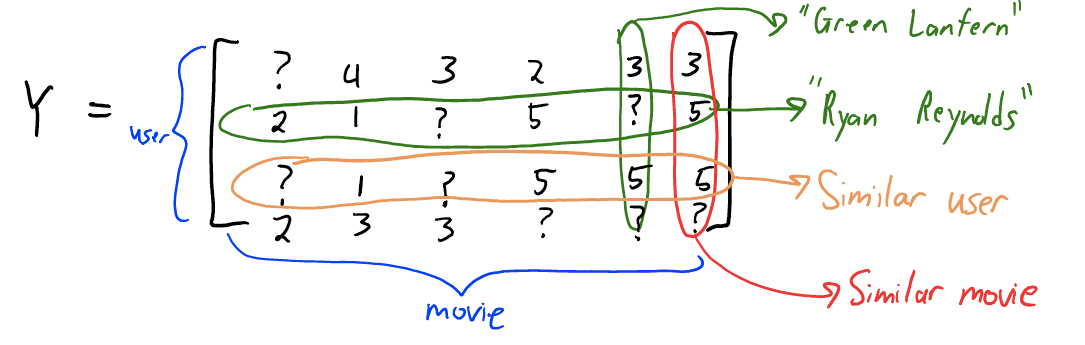
\includegraphics[scale=0.1]{user-item_matrix}
\begin{itemize}
    \item unsupervised learning --- only use labels
    \item latent-factor model: \(y_{ij} \approx w_j^\intercal z_i\)
    \begin{itemize}
        \item \(z_{ic}\) =  ``likes romantic comedies''
        \item \(w_{ic}\) =  ``has Nicholas Cage''
    \end{itemize}
    \item loss function: \(f(Z,W) = \sum\limits_{(i,j) \in R} (w_j^\intercal - y_{ij})^2 + \frac{\lambda_1}{2} ||Z||_F^2 + \frac{\lambda_2}{2} ||W||_F^2\)
    \item add biases: \(y_{ij} \approx \beta + \beta_i + \beta_j + w_j^\intercal z_i\)
    \begin{itemize}
        \item \(\beta \) = global bias
        \item \(\beta_i \) = user-specific bias
        \item \(\beta_j \) = user-specific bias
    \end{itemize}
    \item \(Y_{n \times d} \approx Z_{n \times k} W_{k \times d}\)
\end{itemize}

\subsection{Note}
Problems:
\begin{itemize}
    \item diversity --- how different are the recommendations?
    \item persistence --- how long should recommendations last?
    \item trust --- tell user why you made a recommendation
    \item social recommendation --- what did your friends watch?
    \item freshness --- new and surprising things
\end{itemize}
Content-Based vs. Collaborative
\begin{itemize}
    \item content-based is a linear model and collaborative is a latent-factor model
    \item content-based can predict  on new users/movies, but can't learn about each user/movie
    \item collaborative can learn about each user/movie, but can't predict on new users/movies
\end{itemize}

\section{Multi-Dimensional Scaling (MDS)}
Default Objective
\begin{dmath*}
   f(Z) = \sum_{i=1}^{n} \sum_{j=i+1}^{n} (||z_i - z_j|| - ||x_i - x_j||)^2
\end{dmath*}
Better Objective
\begin{dmath*}
    f(Z) = \sum\limits_{i=1}^{n}\sum\limits_{j=i+1}^{n} d_3(d_2(z_i, z_j) - d_1(x_i, x_j))
\end{dmath*}
\begin{itemize}
    \item \(d_1\) = high-dimensional distance to match
    \item \(d_2\) = low-dimensional distance to control
    \item \(d_3\) = controls how we compare high/low-dimensional distances
\end{itemize}
Choosing \(d_1\), \(d_2\), and \(d_3\)
\begin{itemize}
    \item classic MDS: \(d_1(x_i, x_j) = x_i^\intercal x_j\) and \(d_2(z_i, z_j) = z_i^\intercal z_j\)
    \begin{itemize}
        \item obtains PCA for centered \(x_i\)
        \item not good because it's a linear model
    \end{itemize}
    \item alternative: \(d_1(x_i, x_j) = ||x_i - x_j||_1\) and \(d_2(z_i, z_j) = ||z_i - z_j||\)
    \begin{itemize}
        \item \(z_i\) approximates high-dimensional L1-norm distances
    \end{itemize}
    \item Sammon's mapping to make MDS less crowded by using \emph{weighted} MDS
    \begin{itemize}
        \item \(f(Z) = \sum_{i=1}^{n} \sum_{j=i+1}^{n} (\frac{d_2(z_i,z_j) - d_1(x_i,x_j)}{d_1(x_i,x_j)})^2\)
        \item denominator reduces focus on large distances
    \end{itemize}
\end{itemize}

\section{ISOMAP}
\begin{center}
    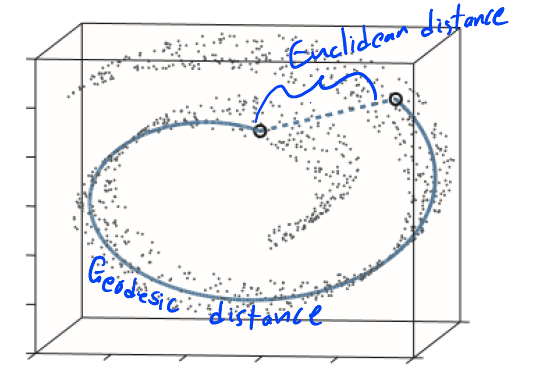
\includegraphics[scale=0.2]{manifold}
\end{center}
\begin{itemize}
    \item PCA/MDS can't discover non-linear manifolds
    \item Geodesic distance (distance through the manifold), is used for low-dimensional manifold
    \item ISOMAP is a latent-factor model for visualizing data on manifolds
\end{itemize}
ISOMAP Procedure \\
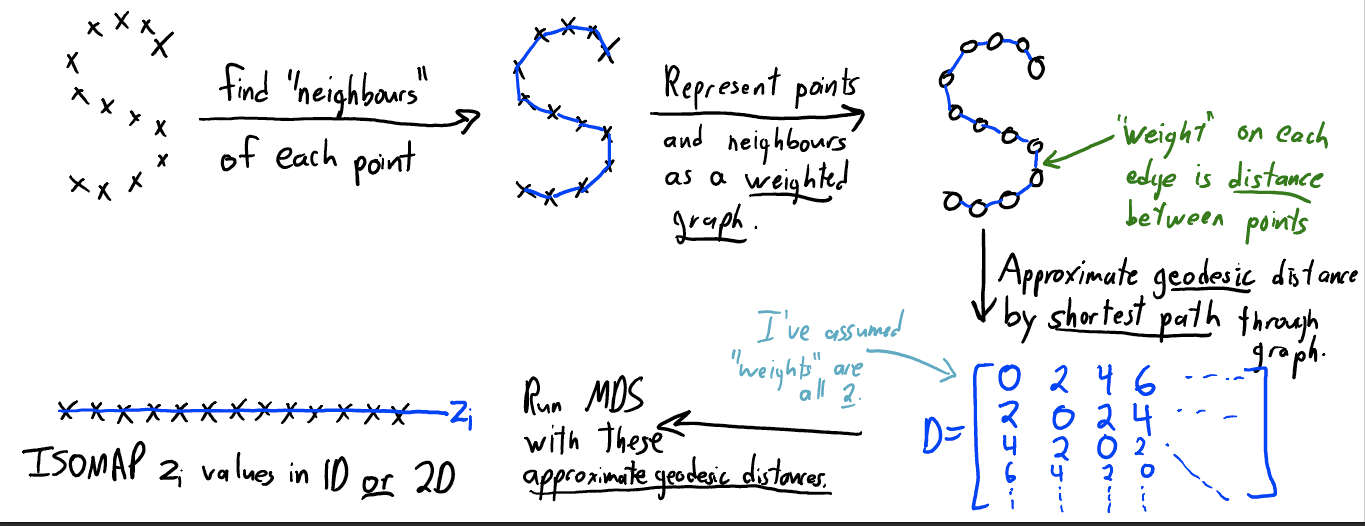
\includegraphics[scale=0.12]{isomap_procedure}

\subsection{Note}
Constructing Neighbour Graph
\begin{itemize}
    \item epsilon graph: convert \(x_i\) to all \(x_j\) within some threshold \(\epsilon \)
    \item KNN graph: connect \(x_i\) to \(x_j\) if \(x_j\) = KNN of \(x_i\) OR \(x_i\) = KNN of \(x_j\)
    \item mutual KNN graph: connect \(x_i\) to \(x_j\) if \(x_j\) = KNN of \(x_i\) AND \(x_i\) = KNN of \(x_j\)
\end{itemize}
ISOMAP vs. t-SNE \\
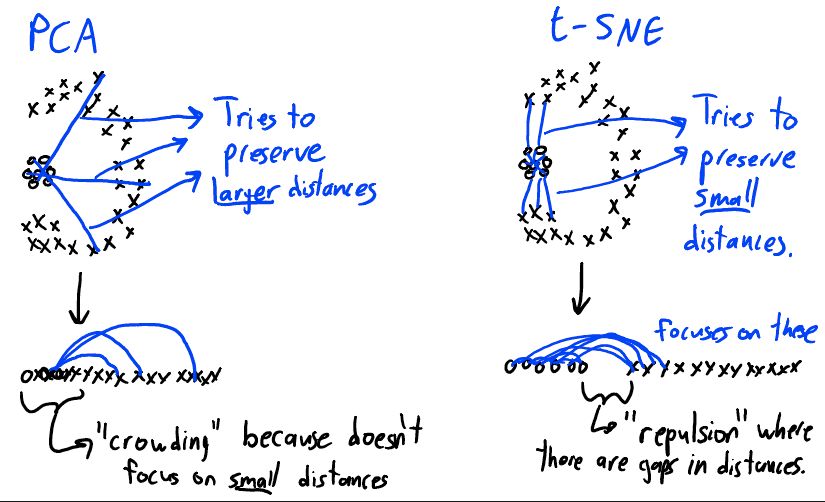
\includegraphics[scale=0.15]{isomap_vs_t-sne}

\section{Neural Networks}
\begin{dmath*}
    f(W^{(1)},W^{(2)}) = \frac{1}{2} \sum_{i=i}^{n} (w^\intercal h(W^{(2)}h(W^{(1)}x_i))-y_i)^2 + \frac{\lambda}{2}||w||^2 + \frac{\lambda_1}{2} ||W^{(1)}||_F^2 + \frac{\lambda_2}{2} ||W^{(2)}||_F^2
\end{dmath*}
\begin{itemize}
    \item \(W^1\) is \(k_1 \times d\), \(W^2\) is \(k_2 \times k_1\), and \(w\) is \(k_2 \times 1\)
    \item \(k \uparrow \) \(\rightarrow \) \(E_{train} \downarrow \text{ but } E_{approx} \uparrow \)
    \item \(\lambda \uparrow \) \(\rightarrow \) \(E_{train} \uparrow \text{ but } E_{approx} \downarrow \)
    \item depth \(\uparrow \) \(\rightarrow \) \(E_{train} \uparrow \text{ but } E_{approx} \downarrow \)
\end{itemize}

Note:
\begin{itemize}
    \item deep learning is sensitive to initialization \(\because\) it's non-convex
\end{itemize}

\subsection{Convolutional Neural Networks}
Motivation:
\begin{itemize}
    \item reduce \# parameters
    \item exploit structure in data
    \item reduce overfitting
\end{itemize}

\section{Math}
Objective functions and derivatives:
\begin{align*}
   f(x) &= \frac{1}{2}\sum\limits_{i=1}^{n} (w^\intercal x_i - y_i)^2 + \frac{\lambda}{2} \sum\limits_{j=1}^{d} w_j^2 \\
   &= \frac{1}{2} ||Xw-y||^2 + \frac{\lambda}{2} ||w||^2
\end{align*}
\begin{itemize}
    \item \(\sum\limits_{i=1}^{n} (w^\intercal x_i - y_i)^2 = \sum\limits_{i=1}^{n} r_i^2 = r^\intercal r = ||r||^2\)
    \item \(||v|| = \sqrt{\sum\limits_{j=1}^{d} v_j^2}\), \(u^\intercal v = \sum\limits_{j=1}^{d} u_j v_j\)
    \item \(||w||^2 = \sum\limits_{j=1}^{d} w_j^2 = \sum\limits_{j=1}^{d} w_j w_j = w^\intercal w \)
\end{itemize}
\begin{align*}
    f(w) &= \frac{1}{2} (Xw-y)^\intercal (Xw-y) + \frac{\lambda}{2} w^\intercal w \\
    &= \frac{1}{2} w^\intercal X^\intercal Xw - w^\intercal X^\intercal y - \frac{1}{2} y^\intercal y + \frac{\lambda}{2} w^\intercal w \\
    \nabla f(x) &= X^\intercal Xw - X^\intercal y + \lambda w = 0 \\
    & \rightarrow (X^\intercal X + \lambda I) w = X^\intercal y
\end{align*}
\begin{itemize}
    \item \(\nabla_w (c) = 0\), \(\nabla_w (w^\intercal b) = b\), \(\nabla_w (\frac{1}{2} w^\intercal A w = Aw\)
\end{itemize}
\begin{itemize}
    \item if \(f(x) = \cdots \frac{\lambda}{2} \sum\limits_{j=1}^{d} w_j v_j\), then \(f(x) = \cdots \lambda w^\intercal v\) and \(\nabla f(x) = X^\intercal Xw - X^\intercal y + \lambda v = 0\)
\end{itemize}
\begin{align*}
    f(x) &= \sum\limits_{i=1}^{n} z_i |w^\intercal x_i - y_i| + \lambda \max_j |w_j|
\end{align*}
\begin{align*}
    f(w) = ||Z(Xw - y)||_1 + \lambda ||w||_{\infty}
\end{align*}
Convexity:
\begin{itemize}
    \item \(f''(x) \geq 0 \Rightarrow \) convex
    \item a convex function multiplied by a non-negative constant is convex
    \item norms and squared norms are convex
    \item \(\exp()\) is convex
    \item sum of convex functions is convex
    \item max of convex is convex
    \item composition of a convex function and linear function is convex
    \item \emph{BUT} composition of a convex function and another convex function may not be convex
\end{itemize}
Maximum Likelihood Estimation (MLE):
\begin{itemize}
    \item minimizing NLL
    \item \(f(x) = - \sum_{i=1}^{n}\log{(p(y_i|x_i,w))}\)
    \item runtime: \(O(nd)\)
\end{itemize}

\section{Plots}
\begin{itemize}
    \item decision tree (1 variable at a time) \\
    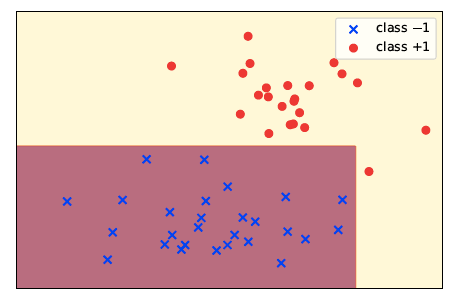
\includegraphics[scale=0.3]{decision_tree_plot}
    \item KNN with \(k=1\) \\
    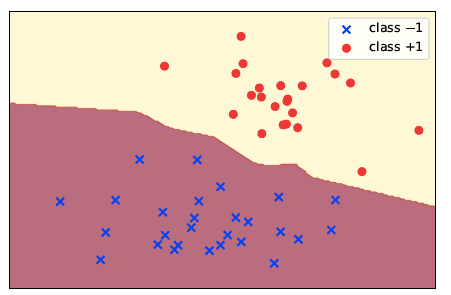
\includegraphics[scale=0.3]{knn_plot}
    \item L2-regularized logistic regression \\
    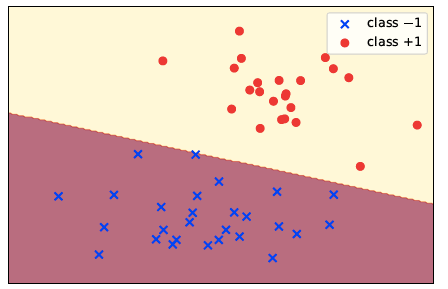
\includegraphics[scale=0.3]{l2_regularized_logistic_regression_plot}
    \item linear SVM (maximizes the margin)\\
    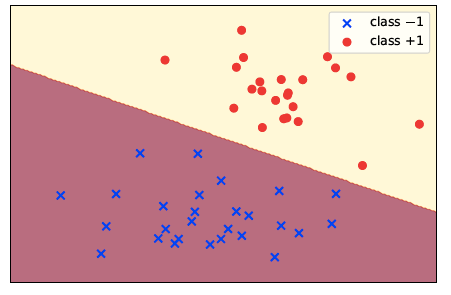
\includegraphics[scale=0.3]{linear_svm_plot}
    \item RBF SVM (blob-like boundaries) \\
    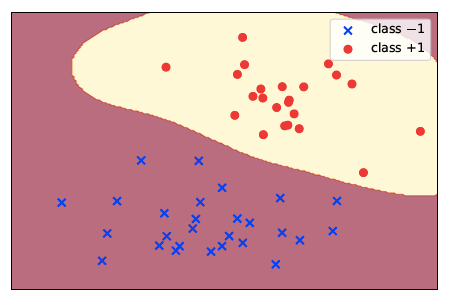
\includegraphics[scale=0.3]{rbf_svm_plot}
    \item neural network using 1 hidden layer and ReLUs \\
    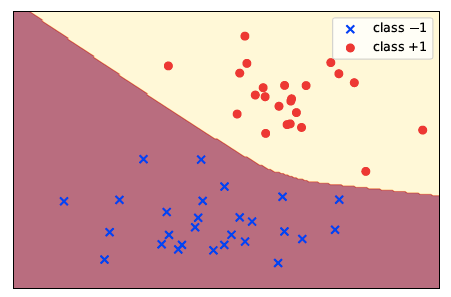
\includegraphics[scale=0.3]{neural_network_plot}
    \item non-regularized L2 norm (not robust) \\
    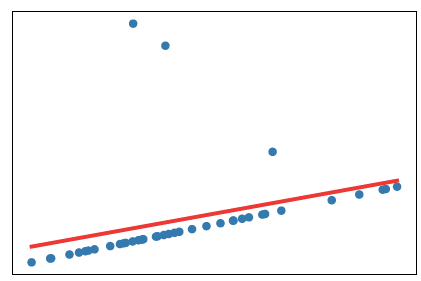
\includegraphics[scale=0.3]{non_regularized_l2_norm}
    \item regularized L2 norm (robust \(\because \) smaller slope) \\
    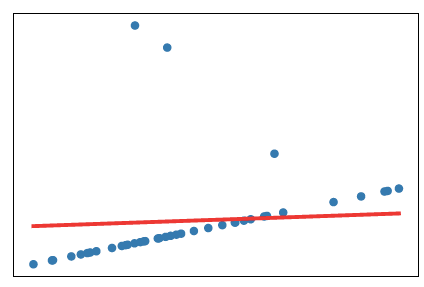
\includegraphics[scale=0.3]{regularized_l2_norm}
    \item L1 norm (robust fit \(\because \) absolute value loss) \\
    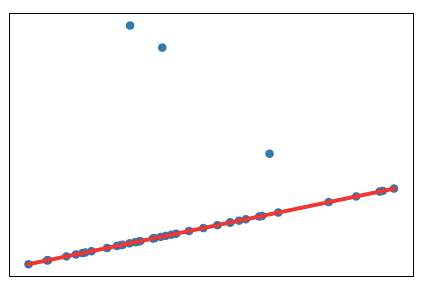
\includegraphics[scale=0.3]{l1_norm}
\end{itemize}

\section{Some Tips}
\begin{itemize}
    \item \textbf{decision stump}: computer error for different stumps then choose the one with the least error
    \item \textbf{randomness of random forest}:
    \begin{itemize}
        \item random subset of data
        \item random subset of features
    \end{itemize}
    \item \textbf{golden rule of ML}: test data should not influence training phase in any way
    \item \textbf{IID assumption}:
    \begin{itemize}
        \item objects from the same distribution
        \item objects sampled independently
    \end{itemize}
    \item \textbf{fundemental trade-off}: \(E_{train} \text{ vs. } E_{approx}\)
    \item \textbf{no free lunch (NFL) theorem}: There is no ``best'' model achieving the best generalization error for every problem.
    \item \textbf{removal of outliers}:
    \begin{itemize}
        \item pro: avoid distortion
        \item con: outliers could be real data
    \end{itemize}
\end{itemize}

\end{multicols*}
\end{document}
